\RequirePackage[l2tabu,orthodox]{nag}
%
\documentclass[12pt, a4paper]{report}
%
\usepackage[utf8]{inputenc}
\usepackage[T1,T2A]{fontenc}
\usepackage[russian]{babel}
%
\usepackage[intlimits]{amsmath}  % Basic math structures
\usepackage{amssymb}  % Extended symbols
\usepackage{amsthm}  % Theorem environment
\usepackage{bm}
%
\usepackage[a4paper,margin=3cm,includefoot,heightrounded]{geometry}
\usepackage[colorlinks,unicode]{hyperref}
\usepackage{layout}
\usepackage{dsfont}
\usepackage{mathrsfs}
\usepackage{mathtools}
\usepackage{multirow}
\usepackage{tikz}
\usepackage{titlesec}
\usepackage{pgf}
\usepackage{pgfplots}
\usepackage{graphicx}
%
\usepackage{wrapfig}
%
\usepackage[backend=biber]{biblatex}
\usepackage{subfiles}
%
\addbibresource{bibliography.bib}
%
\graphicspath{ {./figs/} }
%
\pgfplotsset{compat=1.16}
\usetikzlibrary{babel}
\usetikzlibrary{arrows}
\usetikzlibrary{decorations}
\usetikzlibrary{decorations.markings}
\usetikzlibrary{patterns}
%
%
\titleformat{\chapter}[block]{\normalfont\huge\bfseries\centering}{\S \thechapter.}{20pt}{\Huge}
\newcommand*{\CC}{\mathbb{C}}
\newcommand*{\RR}{\mathds{R}}
\newcommand*{\ZZ}{\mathds{Z}}
\newcommand*{\NN}{\mathds{N}}
\newcommand*{\QQ}{\mathds{Q}}

\newcommand*{\EV}{\mathbf{E}}
\newcommand*{\Var}{\mathbf{D}}
\newcommand*{\PR}{\mathbf{P}}

\newcommand*{\D}{\bm{D}}
\newcommand*{\R}{\bm{R}}
\newcommand{\BraceThree}{%
	\multirow{3}{*}{$\left\{\begin{array}{@{}l@{}} \null \\ \null \\ \null\end{array}\right.$}%
}

\newcommand{\BraceTwo}{%
	\multirow{2}{*}{$\left\{\begin{array}{@{}l@{}} \null \\ \null\end{array}\right.$}%
}

\renewcommand\qedsymbol{$\blacksquare$}

\theoremstyle{plain}
\newtheorem{Th}{Теорема}
\newtheorem*{Th*}{Теорема}
\newtheorem{Lem}{Лемма}
\newtheorem*{Lem*}{Лемма}
\newtheorem*{St}{Утверждение}
\newtheorem*{Prop}{Свойства}

\theoremstyle{definition}
\newtheorem*{Def}{Определение}
\newtheorem*{Ex}{Пример}
\newtheorem*{Nam}{Обозначение}
\newtheorem*{Agr}{Договоренность}

\theoremstyle{remark}
\newtheorem*{Rem}{Замечание}
\newtheorem*{Probl}{Упражнение}

\renewcommand{\proofname}{Доказательство}
\addto\captionsrussian{
	\renewcommand{\proofname}{Доказательство}
}

\newenvironment{amatrix}[1]{%
	\left(\begin{array}{@{}*{#1}{c}|c@{}}
	}{%
	\end{array}\right)
}

\DeclareMathOperator*{\Res}{Res}
\DeclareMathOperator{\PE}{E}
\DeclareMathOperator{\PP}{P}

\renewcommand{\Re}{\operatorname{Re}}
\renewcommand{\Im}{\operatorname{Im}}

\DeclareMathOperator*{\argmin}{arg\,min}
%
\begin{document}
%
\thispagestyle{empty}
\sloppy
\begin{titlepage}
\begin{center}
Московский государственный университет имени~М.~В.~Ломоносова\\
механико-математический факультет\\
кафедра математической статистики и случайных процессов\\

\centering
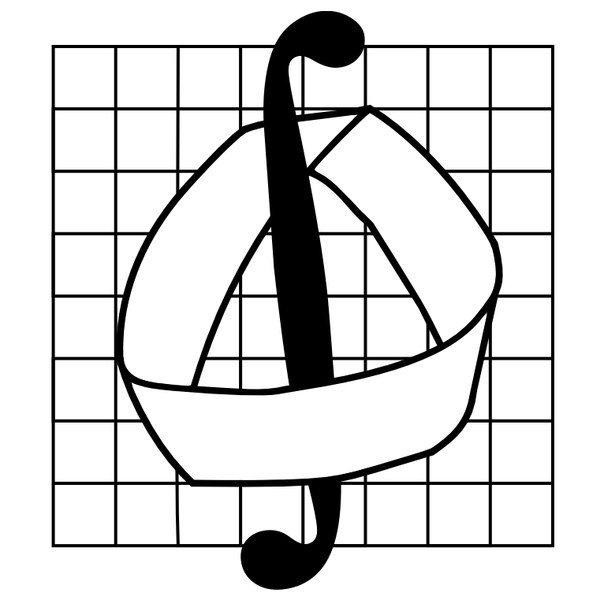
\includegraphics[width=0.3\textwidth]{mechmath.jpg}

\vspace*{100pt} Курсовая работа\\студента 503 группы \\
Купрякова Василия Юрьевича
\\
\vspace{10pt} {\Large{\textbf{Непараметрическая вейвлет-оценка плотности мультипликативно зашумленных данных}}\\}

\vspace*{40pt}

\begin{flushright}
Научный руководитель:\\ с.н.с., к.ф.-м.н.\\  Шкляев Александр Викторович\\
\end{flushright}

\vspace*{\fill} Москва, 2021
\end{center}
\end{titlepage}
\clearpage
%
\tableofcontents
%
\subfile{chapters/introduction}
%
\subfile{chapters/inverse-laplace}
%
\subfile{chapters/mellin-solution}
%
\subfile{chapters/fredholm}
%
\subfile{chapters/evaluation}
%
\subfile{chapters/multilength}
%
\subfile{chapters/results}
%
\section{Правильная часть ряда Лорана для $f(z) = e^{az} e^{-1/(2s^2)} e^{n/s}$}
\begin{Th*}
Пусть $k \ge 0$; пусть
\[
    f(z) = e^{az} e^{-1/(2s^2)} e^{b/z}
\]
Тогда $k$-й член ряда Лорана для $f$ равен
\[
    \sum_{l=0}^{\infty}
    \sum_{m=0}^{\infty} \frac{a^{2m+k+l} / \left( -2 \right)^m}{(2m+k+l)!\,m!} \\
    \frac{n^l}{l!}
\]
\end{Th*}
\begin{proof}
Определим
\begin{align*}
    & g(t) = e^{az} e^{-1/(2s^2)} \\
    & h(t) = e^{b/z}
\end{align*}
Обе функции голоморфны в $\CC \setminus \{0\}$. Поэтому их ряды сходятся абсолютны и мы можем умножить ряды по Коши, чтобы получить ряд Лорана для $f$.

У функции $e^{n/s}$ правильная часть константна.
Поэтому, согласно теореме о правильной части произведения голоморфной функции и функции с константной правильной частью, 
нам достаточно знать только правильную часть разложения функции $g$, которую мы нашли в предыдущей теореме.

Пусть $\{\alpha_n\}_{n=-\infty}^\infty$ --- коэффициенты для $g$, а $\{\beta_n\}_{n=-\infty}^0$ --- коэффициенты для $h$, а $\{\gamma_n\}_{n=-\infty}^\infty$ --- коэффициенты $f$.
Для наглядности, приведем формулу $k$-го члена их произведения, где $k \ge 0$:
\[
    \gamma_k =
    \sum_{l=-\infty}^{0} \alpha_{k-l} \beta_l =
    \sum_{l=0}^{\infty} \alpha_{k+l} \beta_{-l}
\]
Приведем также формулы для $\alpha_k$ и $\beta_{-k}$:
\begin{align*}
    & \alpha_k = \sum_{m=0}^{\infty} \frac{a^{2m+k} / \left( -2 \right)^m}{(2m+k)!\,m!} \\
    & \beta_{-k} = \frac{n^k}{k!}
\end{align*}
Подставим $\alpha_k$ и $\beta_{-k}$ в формулу для $\gamma_k$:
\[
    \gamma_k =
    \sum_{l=0}^{\infty} \alpha_{k+l} \beta_{-l} =
%
    \sum_{l=0}^{\infty}
    \sum_{m=0}^{\infty} \frac{a^{2m+k+l} / \left( -2 \right)^m}{(2m+k+l)!\,m!} \\
    \frac{n^l}{l!}
\]
\end{proof}

%
\printbibliography
\end{document}
